% ============================================================================
% SYSTEM ARCHITECTURE
% ============================================================================
\section{System Architecture}

\subsection{Network Topology}

\begin{figure}[H]
\centering
\begin{tikzpicture}[
    node distance=1.5cm,
    box/.style={draw, rectangle, rounded corners, minimum width=3cm, minimum height=1.2cm, align=center},
    arrow/.style={->, thick, >=stealth}
]
    % External Internet
    \node[box, fill=blue!20] (internet) {External Internet};

    % WiFi modes explanation
    \node[right=1cm of internet, font=\small, align=left] (wifi_note) {
        WiFi STA: Connect to home/office WiFi\\
        WiFi AP: Create \texttt{star-robot} network
    };

    % Controller App
    \node[box, fill=green!20, below left=3.5cm and 4cm of internet] (controller) {Controller App\\(PWA - any device)};

    % RPi5
    \node[box, fill=orange!20, minimum width=5cm, minimum height=2cm, below=2cm of internet] (rpi) {
        \textbf{Raspberry Pi 5}\\
        Spring Boot Gateway\\
        ROS 2 Jazzy / SLAM
    };

    % Hand Controller
    \node[box, fill=green!30, below left=2cm and 0cm of rpi] (hand) {Hand Controller\\(local network)};

    % ESP32
    \node[box, fill=red!20, below=2cm of rpi] (esp32) {ESP32-S3\\Motor Control\\1kHz PID loop};

    % LiDAR
    \node[box, fill=purple!20, below right=2cm and 0cm of rpi] (lidar) {RPLiDAR C1\\LiDAR 360\textdegree};

    % Connections
    \draw[arrow] (internet) -- node[right, font=\small] {WiFi STA} (rpi);
    \draw[arrow, <->] (controller) -- node[above, font=\small, yshift=0.15cm] {gRPC/GraphQL} (rpi);
    \draw[arrow, <->] (hand) -- node[left, font=\small] {WiFi AP} (rpi);
    \draw[arrow, <->] (rpi) -- node[left, font=\small] {SPI + TCP} (esp32);
    \draw[arrow, <->] (rpi) -- node[right, font=\small] {UART} (lidar);

\end{tikzpicture}
\caption{Complete Network Topology}
\end{figure}

\subsection{Dual WiFi Mode Operation}

The Raspberry Pi 5 operates in \textbf{simultaneous dual WiFi mode}:

\begin{enumerate}
    \item \textbf{Station (STA) Mode}: Connects to external internet for remote access
    \begin{itemize}
        \item Enables control from anywhere with internet access
        \item Allows firmware updates and remote debugging
    \end{itemize}

    \item \textbf{Access Point (AP) Mode}: Creates local \texttt{star-robot} network
    \begin{itemize}
        \item Provides low-latency local control
        \item ESP32 connects to this network for TCP fallback
        \item Hand controller connects for direct operation
    \end{itemize}
\end{enumerate}

\subsection{Software Stack Overview}

\begin{figure}[H]
\centering
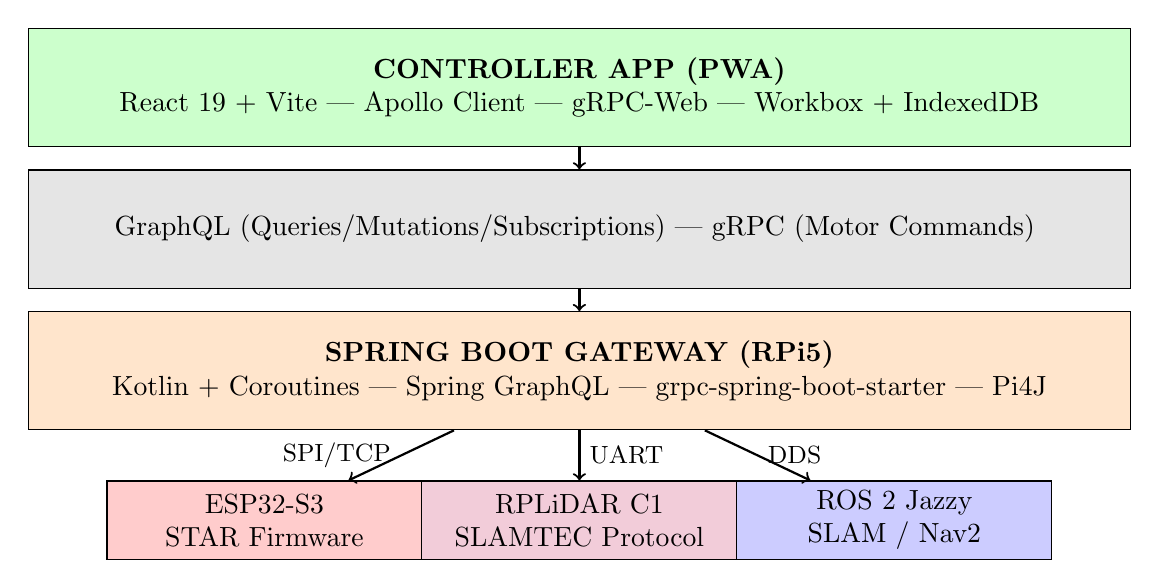
\begin{tikzpicture}[
    layer/.style={draw, rectangle, minimum width=14cm, minimum height=1.5cm, align=center},
    sublayer/.style={draw, rectangle, minimum width=4cm, minimum height=1cm, align=center}
]
    % Controller App Layer
    \node[layer, fill=green!20] (frontend) at (0,6) {
        \textbf{CONTROLLER APP (PWA)}\\
        React 19 + Vite | Apollo Client | gRPC-Web | Workbox + IndexedDB
    };

    % Protocol Layer
    \node[layer, fill=gray!20] (protocol) at (0,4.2) {
        GraphQL (Queries/Mutations/Subscriptions) | gRPC (Motor Commands)
    };

    % Gateway Layer
    \node[layer, fill=orange!20] (gateway) at (0,2.4) {
        \textbf{SPRING BOOT GATEWAY (RPi5)}\\
        Kotlin + Coroutines | Spring GraphQL | grpc-spring-boot-starter | Pi4J
    };

    % Hardware Layer
    \node[sublayer, fill=red!20] (esp32) at (-4,0.5) {ESP32-S3\\STAR Firmware};
    \node[sublayer, fill=purple!20] (lidar) at (0,0.5) {RPLiDAR C1\\SLAMTEC Protocol};
    \node[sublayer, fill=blue!20] (ros) at (4,0.5) {ROS 2 Jazzy\\SLAM / Nav2};

    % Connections
    \draw[->, thick] (frontend) -- (protocol);
    \draw[->, thick] (protocol) -- (gateway);
    \draw[->, thick] (gateway) -- node[left, font=\small] {SPI/TCP} (esp32);
    \draw[->, thick] (gateway) -- node[right, font=\small] {UART} (lidar);
    \draw[->, thick] (gateway) -- node[right, font=\small] {DDS} (ros);

\end{tikzpicture}
\caption{Software Stack Architecture}
\end{figure}
